\documentclass[12pt, a4paper]{article}
\usepackage{amssymb}

\makeatletter
\begingroup\endlinechar=-1\relax
       \everyeof{\noexpand}%
       \edef\x{\endgroup\def\noexpand\homepath{%
         \@@input|"kpsewhich --var-value=HOME" }}\x
\makeatother

\def\overleafhome{/tmp}% change as appropriate
\usepackage{fontspec}
\ifx\homepath\overleafhome
\setmonofont[Path = ../]{CONSOLA.TTF}[
BoldFont=CONSOLAB.ttf,
ItalicFont=CONSOLAI.ttf,
BoldItalicFont=CONSOLAZ.ttf
]
\else
\setmonofont{Consolas}
\fi

\usepackage[title]{appendix}
\usepackage[onehalfspacing]{setspace}
\usepackage{subfigure}
\parskip=1mm plus 1pt
\usepackage{indentfirst}
\usepackage{forest}
\usepackage[export]{adjustbox}

\usepackage[section]{placeins}

\usepackage{xcolor}
\usepackage{algorithm}
\usepackage{algorithmic}
\usepackage{hyperref}
\hypersetup{
unicode=true,          % non-Latin characters in Acrobat’s bookmarks
pdftitle={},    % title   
%pdfauthor={爱让一切都对了},     % author   
%pdfcreator={爱让一切都对了},
%pdfproducer={OpenOffice.org 3.3},
breaklinks=true,
colorlinks=true,       % false: boxed links; ture: colored links
linkcolor=blue,          % color of internal links   
citecolor=blue,        % color of links to bibliography  
filecolor=magenta,      % color of file links   
urlcolor=cyan,           % color of external links  
}

\usepackage{url}
\def\UrlBreaks{\do\A\do\B\do\C\do\D\do\E\do\F\do\G\do\H\do\I\do\J\do\K\do\L\do\M\do\N\do\O\do\P\do\Q\do\R\do\S\do\T\do\U\do\V\do\W\do\X\do\Y\do\Z\do\[\do\\\do\]\do\^\do\_\do\`\do\a\do\b\do\c\do\d\do\e\do\f\do\g\do\h\do\i\do\j\do\k\do\l\do\m\do\n\do\o\do\p\do\q\do\r\do\s\do\t\do\u\do\v\do\w\do\x\do\y\do\z\do\0\do\1\do\2\do\3\do\4\do\5\do\6\do\7\do\8\do\9\do\.\do\@\do\\\do\/\do\!\do\_\do\|\do\;\do\>\do\]\do\)\do\,\do\?\do\'\do+\do\=\do\#}

\usepackage{listings}
% JavaScript
\lstdefinelanguage{JavaScript}{
  morekeywords={typeof, new, true, false, catch, function, return, null, catch, switch, var, if, in, while, do, else, case, break, const, let, var},
  morecomment=[s]{/*}{*/},
  morecomment=[l]//,
  morestring=[b]",
  morestring=[b]'
}
\lstset{
%  %行号
%  %numbers=left,
%  %背景框
%  %framexleftmargin=10mm,
%  %frame=none,
%  %背景色
%  %backgroundcolor=\color[rgb]{1,1,0.76},
%  %样式
  keywordstyle=\color{blue}\bfseries,
%  identifierstyle=\bf,
%  numberstyle=\color[RGB]{0,192,192}, %行号的样式
  commentstyle=\it\color[RGB]{0,96,96},
  stringstyle=\ttfamily\color[RGB]{128,0,0},
%  %显示空格
%  %showstringspaces=false,
  basicstyle=\ttfamily\footnotesize, %修正大写字母间距过小
  columns=flexible, %修正大写字母间距过小
  breaklines=true, %对过长的代码自动换行
%  escapechar=!,
%  morekeywords={BEGIN}
  upquote=true,
  language=JavaScript,
  tabsize=4
}


\newcommand{\code}[1]{\texttt{#1}}
\title{CS 188 Final Project Report}
\author{Weikeng Yang\\405346443 \and
Yingzhe Hu\\505366341 \and
Qiqi Gu\\604253019 \and
Dongyao Liang\\705313832 \and
Shuhua Zhan\\705190671}
\date{Team name: Random\\[2mm]March 20, 2020}

\usepackage[numbers]{natbib}
\setcitestyle{square}

\usepackage{graphicx}
\usepackage{pgfkeys}

\begin{document}

\maketitle

\tableofcontents
\newpage

\newcommand{\theproject}{Five Peas Flight Search}
\section{Summary}
This report evaluates Team Five Peas in a Pod's project, Five Peas Flight Search. We have the source code of the client side. The application talks to Google Firebase server while configuration files of Firebase is missing from the repository. %Therefore we focus on evaluating the client side.

The application has been deployed to Google App Engine, accessible via \url{https://five-peas-flight-search.appspot.com}. 
%We will evaluate the security of the source code and the server deployment.

We contacted the team, and they sent us an updated design report on \url{https://docs.google.com/document/u/1/d/1EGwWqXqnp9lyWc8q5S34Y_EgQw0M8s2LtmIN8-LypG8/edit?usp=drive_web&ouid=107934347927820032084}, which is different than the one the professor sent us. We evaluate based on the updated version.

We mainly run the application locally in that we can modify the code and see the impact. However, the application was designed to run at \url{https://five-peas-flight-search.appspot.com}, this particular address. If we run it at a different address, Login, Firebase, and some other functions don't work. Therefore sometimes we have to use the deployed version.

%The project uses a number of external components, among which, Bootstrap 4.4.1 and vuejs 2.6.11 are fairly new. People may not have enough time to evaluate their security implications. Only the code that loads bootstrap has the \code{integrity} and \code{crossorigin} attributes. We suggest to add them to other \code{<script>} elements.\textsuperscript{\cite{html-standard-script}}

In code review, we used candidate point strategy, and use debugger to better understand the execution flow. 

We founds security vulnerabilities, including the overwritten escape function, maxlength and storage vulnerability, and bugs, including dash issue in airport names, unable to load large saved itinerary.


%Requirement: A brief summary of your findings, including the approach(es) you took and what you learned. This should be at a high level (e.g., "Working from the design document, we decided to perform code review using the following techniques, supplemented by the following kinds of testing") and should include some conclusion about the security of the system (e.g., "Our analysis showed that the mitigations used to address security concerns in our system were effective," or "Our analysis reveals fatal security flaws that could be remediated in the following ways," or a statement of similar nature).   For evaluation of the other team’s project, remember that your goal is not to criticize their efforts, but to determine whether they achieved sufficiently secure results and to suggest improvements if they did not. 

\section{Security Evaluation Plan}

%Requirement: A description of your plan for the security evaluation, including steps to be taken, tools or approaches used, work assignments, and a schedule. Since it is likely that your plan required some adjustments, you should discuss the degree to which you followed your plan versus deviating from it, as well as explanations for such deviations.  

As the instructor mentioned in the lecture, we are going to evaluate Five Peas' project security according to the following steps.

\begin{itemize}
    \item Security Design Review (03/07/2020 - 03/09/2020)
    \item External Components Review (03/09/2020)
    \item Code Review (03/10/2020 - 03/11/2020)
    \item Tool Testing (03/12/2020 - 03/13/2020)
    \item Data Security, DDOS attack, and SSL Test (03/12/2020) 
\end{itemize}
    

\section{Security Evaluation Results}

\subsection{Security Design Review}
\begin{figure}[ht]
\centering
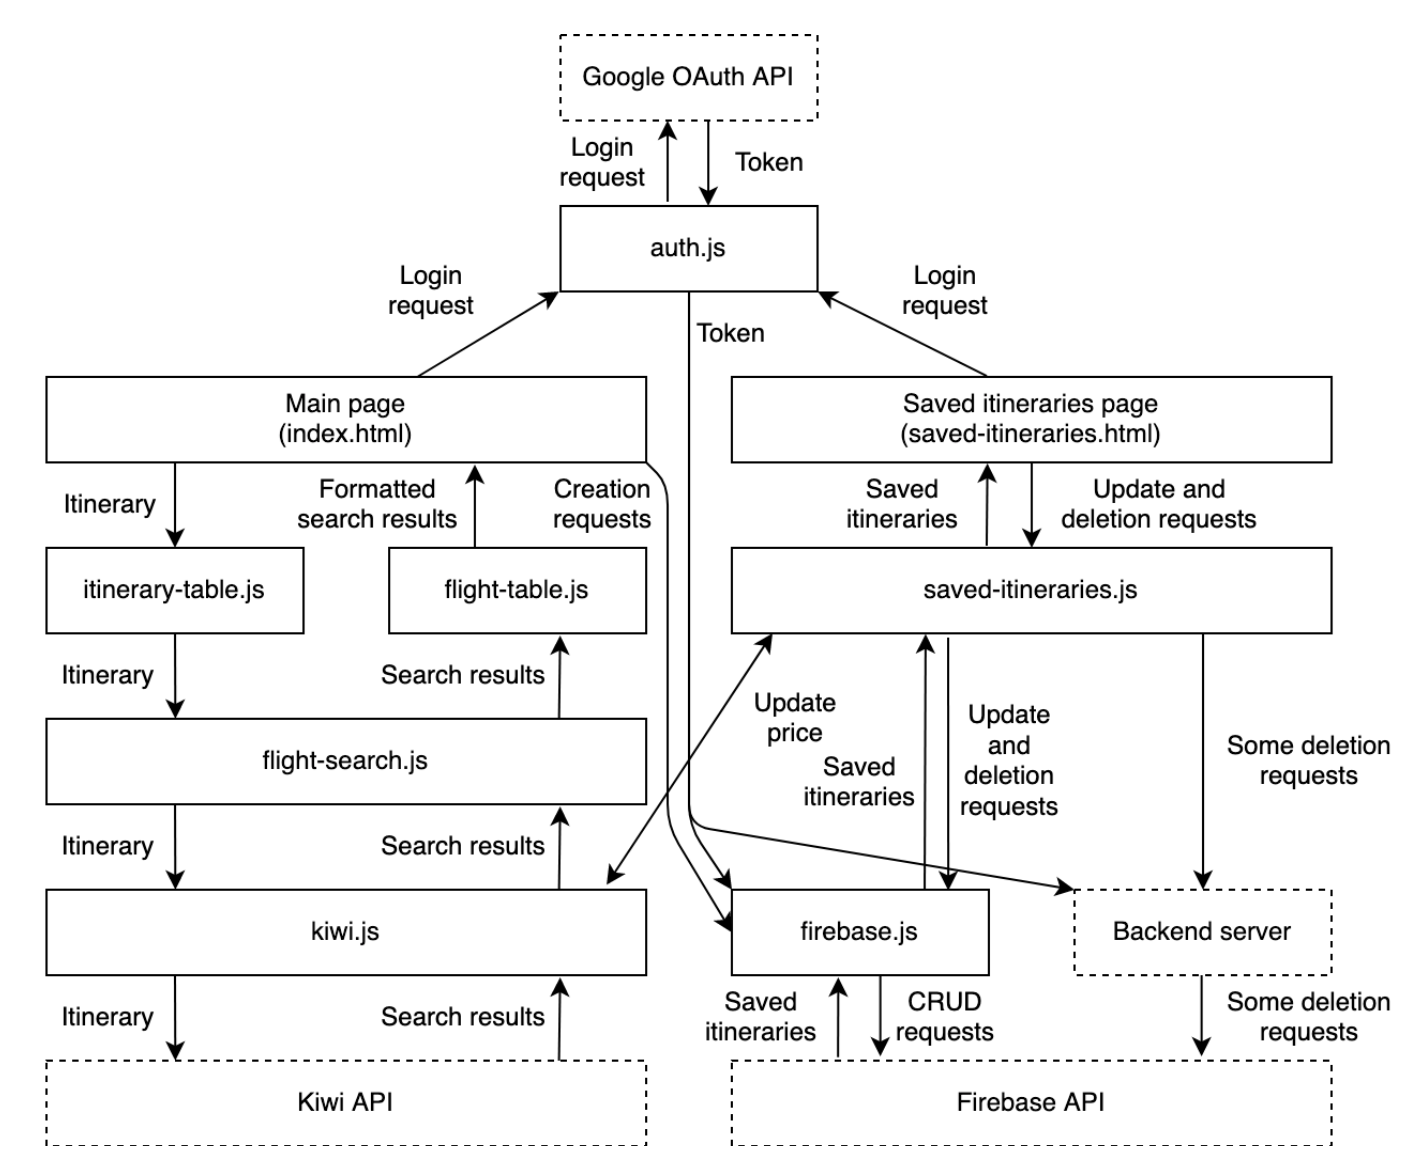
\includegraphics[width=0.8\textwidth]{design_structure.png}
\caption{Design Diagram}
\label{fig:design_diagram}
\end{figure}
\subsubsection{Design Review Summary}
Five Peas Flight Search is a versatile flight search engine that provides users with flight itinerary according to the departure city and the arrival city of their inputs. As it is shown in the graph, the design is divided into two parts. Front-end interact with Kiwi API and CRUD operations with \code{Firebase} and back-end constructed mainly by \code{app.js} which serves the front-end files and exposes one endpoint to control deletion of a specific itinerary. With the log-in feature powered by Goolge Sign-In API, users can save itineraries and the history prices into \code{Firebase}. \code{Firebase} stores the data of clients (logging in and saved information). It deals with file creation and deletion. 

If users choose not to log in,  log-in request would not be sent. \code{itinerary-table.js} manages users' input on the website table. \code{flight-table.js} would display the search results receiving from \code{flight-search.js} and provides a link to redirect to the Kiwi page. \code{flight-search.js} gets the input from use via \code{itinerary-table.js} and pass into \code{kiwi.js}; \code{kiwi.js} generates the results from Kiwi website and then sends back the results to \code{flight-table.js} for display. \code{kiwi.js} is the file that takes the itinerary information as input and sent to formats a request to Kiwi and searches for results with the users' input directly on Kiwi website.

For logged-in users, \code{saved-itineraries.html} is the web page file to check the saved itineraries. \code{saved-itineraries.\linebreak[1]js} calls \code{auth.js} to determine whether or not a user is authenticated and if yes, display the saved itineraries information from Firebase App by calling \code{firebase.js} (handles connection with Firebase App for users and auth.js).

Therefore, based on the results we get above after a high level of files and code review, our team believes that the prototype of the website largely matches the design.
\subsubsection{Threats}
A number of potential threats might be evolved in this projects such as DDoS, XSS with JavaScript, incorrect use of Firebase. Our team believe that SQL injections and XSS might be at highest risks; the following would be DDoS attack and incorrect usage of Firebase. 

Even though in the project design, Five Peas developers believe that with the use of Google Cloud, the website can be free from DDoS attack, but it's not usually the case. One of the reasons is that Google Cloud function only can prevent DDoS attacks under layer 4 in TCP/IP. Hacker can still send huge amounts of traffic in HTTP to attack your API \cite{Google-DDoS}. In addition, although Google cloud is powerful enough to handle massive DDos attacks on or above layer 4 ( unless the infrastructure of Google crashed), the website company would still need to pay for the all the traffic and computing time spent from the attack, which would costs a significant amount of money.

Cross-Site Scripting usually happens when a website allows users to upload information. If a malicious hacker sends a script to attack the website with these upload functions, the website could be in great danger and it will possibly affect on the users side as well.
While evaluating the design, we see that users are not allowed to upload anything to the website rather than saving some itinerary information generated from the Kiwi website. Therefore, our team believes that the product has a low possibility of having XSS problems from website function. Since the project uses JavaScript, XSS is usually evolved, which will be discussed more in External Components Reviews session.

Sometimes using Firebase may not be secure because a lot of developers may not follow the security rules to protect their database. Therefore as we looked into Firebase security rule \cite{firebase} and the file \code{firebase.js}, we found that the design has followed Firebase security rules and when reading from the database, it checked if the user requesting data is authenticated by calling the function \code{checkAuth()} beforehand and it only allows the authenticated users (after logging in) to see their own documents rather the whole list of documents. Since we know that there are many limits when doing complicated queries using Firebase, however, as our team look more into the information it’s storing, the website does not query complicated data and does not need the function of searching or filtering information from the database, therefore it should be adequate to use Firebase.

Overall, after a brief design review of the website, our team believes that Five Peas does a good job on preventing most of the security issues by using Google Cloud and Firebase. The vulnerability of SQL injection has been greatly reduced, but there are still potential vulnerabilities of XSS due to JavaScript.


\subsection{External Components Review}
\label{dependency-evaluation}

%Google app engine

%Firebase

%Kiwi API

%Google Client API

%nodejs

%Firebase security rules - not accessible

%admin?

%auth.js, use localstorage

%itinerary-table.js

\subsubsection{JavaScript}
JavaScript is a high-level programming language with dynamic typing and first-class functions. It doesn't have buffer overflow issues. It has integer overflow problems.

JavaScript is executed by browser JavaScript engines. Ideally we should look into the JavaScript engines and make sure Five Peas Flight Search doesn't use vulnerable structures. However, because major browser manufactures\textsuperscript{\cite{chrome-update}} keep many bug details secret, and due to resource constraints, we don't look at the JavaScript engine vulnerabilities.

The common vulnerabilities in JavaScript application are Cross Site Scripting (XSS), Cross-Site Request Forgery (CSRF), Server-side JavaScript Injection (SSJI), etc. 

To avoid XSS, one would avoid inserting HTML directly into the document. We will use Candidate Point strategy to check if any code manipulates HTML directly. What's more, we will check if the project uses \code{eval}, or put untrusted input to \code{setInterval}, \code{setTimeout}, \code{new Function}, and other functions, as suggested in \cite{secure-javascript}.



%Using encodeURIComponent()



%instead, programmatically create DOM nodes and append them to the DOM. This means avoiding .html(), .innerHTML, and other related functions, and instead using .append(), .prepend(), .before(), .after(), and so on.

% Note: It’s technically faster to insert HTML, because the browser is optimized to parse HTML. 

% https://wpvip.com/documentation/vip-go/vip-code-review/javascript-security-best-practices/

% This is the main reason why OWASP recommends never to store sensitive information in LocalStorage, SessionStorage



% 3- Client-side Logic And Data Storage
% 4) 

% https://www.algoworks.com/blog/security-concerns-with-javascript-development/


\subsubsection{Front-end Libraries}
Five Peas Flight Search uses Materialize (\url{https://materializecss.com/}) framework version 1.0.0, released on Sep 9, 2018. In this version, XSS can arise when user input is provided to the \code{autocomplete} component or the \code{tooltip} component.\textsuperscript{\cite{materialize-vulnerabilities}}

Five Peas Flight Search uses Google Fonts. This service is versionless. \cite{google-fonts-privacy} warns a privacy concern that Google APIs Terms of Service allows Google to track users of the sites using Google Fonts. 

Five Peas Flight Search uses Google Sign-In JavaScript client (referred as gapi, \url{https://developers.google.com/identity/sign-in/web/reference}). This service is versionless. We didn't find any security issues in gapi.


\subsubsection{Firebase}
Based on their project design and code review, Firebase really plays an important role in their project. They achieve the security guaranteed by Google in DDoS protection and secure token generation. Furthermore, authentication and registering of the user is entirely handled from the client to Firebase. All user data is stored entirely in Firebase, with the client rendering the data pulled from the Firebase API. 

Firebase is a mobile and web application development platform developed by Firebase, Inc. It offers a variety of development services, such as Firebase Auth and database. Firebase Auth is a service that can authenticate users using only client-side code. It supports social login providers Facebook, GitHub, Twitter and Google. Additionally, it includes a user management system whereby developers can enable user authentication with email and password login stored with Firebase.

On one hand, we think that it's a good idea for them to use Firebase to escort their APP. They can avoid many software security problems and pay more attention to other parts. On the other hand, if developers haven't correctly secured their Firebase database, a simple web request can retrieve its entire contents. Data is exposed probably not by flaws in an application's code but by the development team's failure to properly secure the back end. The reason that it's so prevalent among apps using Google Firebase is that there is no database security turned on by default.

While most applications tend to have security and privacy settings turned on by default, a development platform can be difficult to learn and awkward to use if the security settings are turned on at the beginning of the development cycle, slowing down the initial development phases while the code and functionality are being tested. Anything that slows down development is likely to put developers off using a particular platform.

As a default Firebase database has no security, it's the development team's responsibility to correctly secure the database prior to it storing real data. In Google Firebase, this is done by requiring authentication and implementing rule-based authorization for each database table. The configuration and security controls for any sensitive data also need to be checked using vulnerability scanners and pen test tools to verify that they have been implemented effectively.



  <script src="https://www.gstatic.com/firebasejs/7.9.1/firebase-app.js" defer></script>
  
  <script src="https://www.gstatic.com/firebasejs/7.9.1/firebase-auth.js" defer></script>
  
  <script src="https://www.gstatic.com/firebasejs/7.9.1/firebase-firestore.js" defer></script>
  

\subsection{Code Review}
To run the application, it should be deployed to a web server. PyCharm or WebStorm will create a temporary web server. If a browser opens the local \code{public/index.html} directly, some functions, including the Google Sign in, do not work. Therefore, we use the former method to run the application and perform our code review. Figure \ref{fig:run} shows how to run it in PyCharm.

\begin{figure}
\centering
\subfigure[Use PyCharm or WebStorm to run index.html as the IDE will create a temporary web server.]{
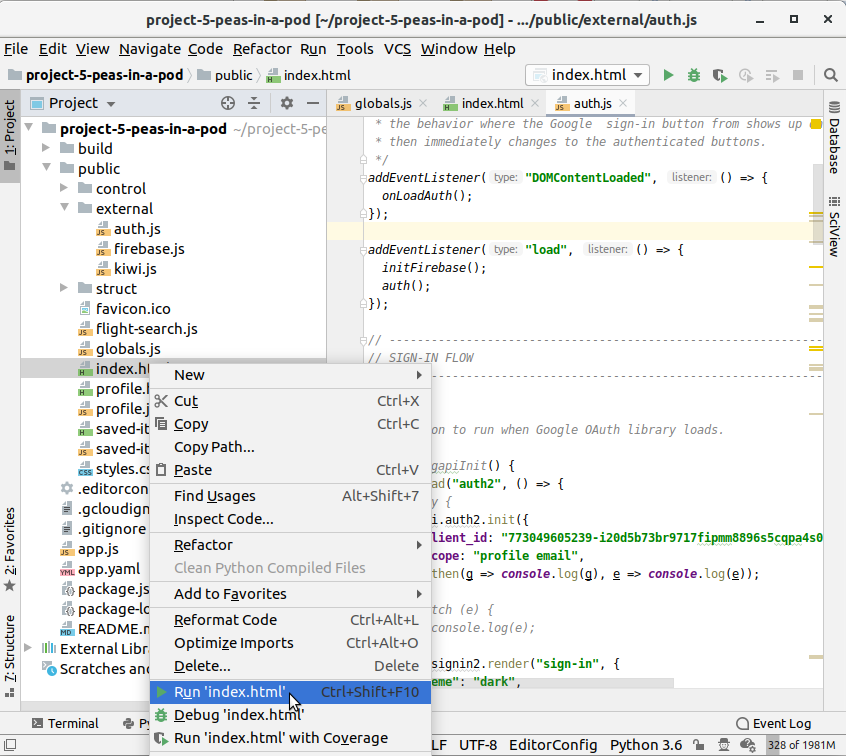
\includegraphics[width=0.8\textwidth]{run.png}
}
\subfigure[The interface of the web application. If a browser opens index.html from local file system, the Sign in button disappears.]{
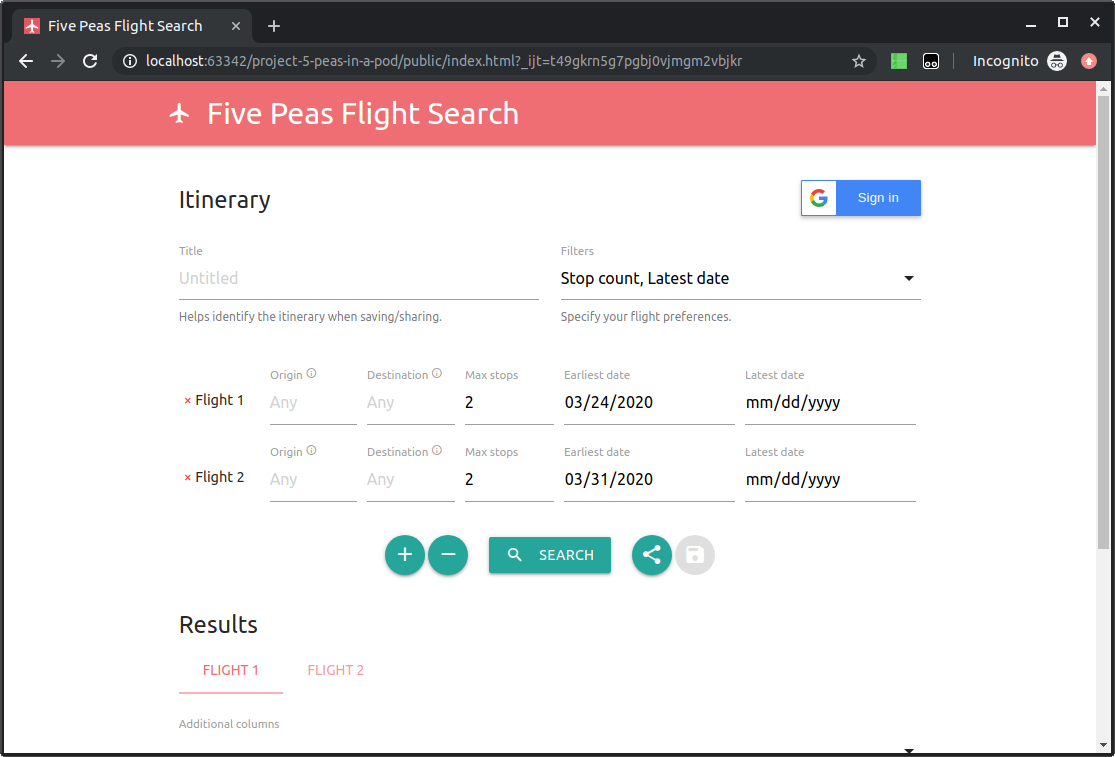
\includegraphics[width=0.8\textwidth]{interface.png}
}
\label{fig:run}
\end{figure}

% We also used debugger to better understand the execution flow. Figure \ref{fig:debugger} verifies \code{itable.loadFromItinerary} is used to show the search table.

% \begin{figure}[ht]
% \centering
% 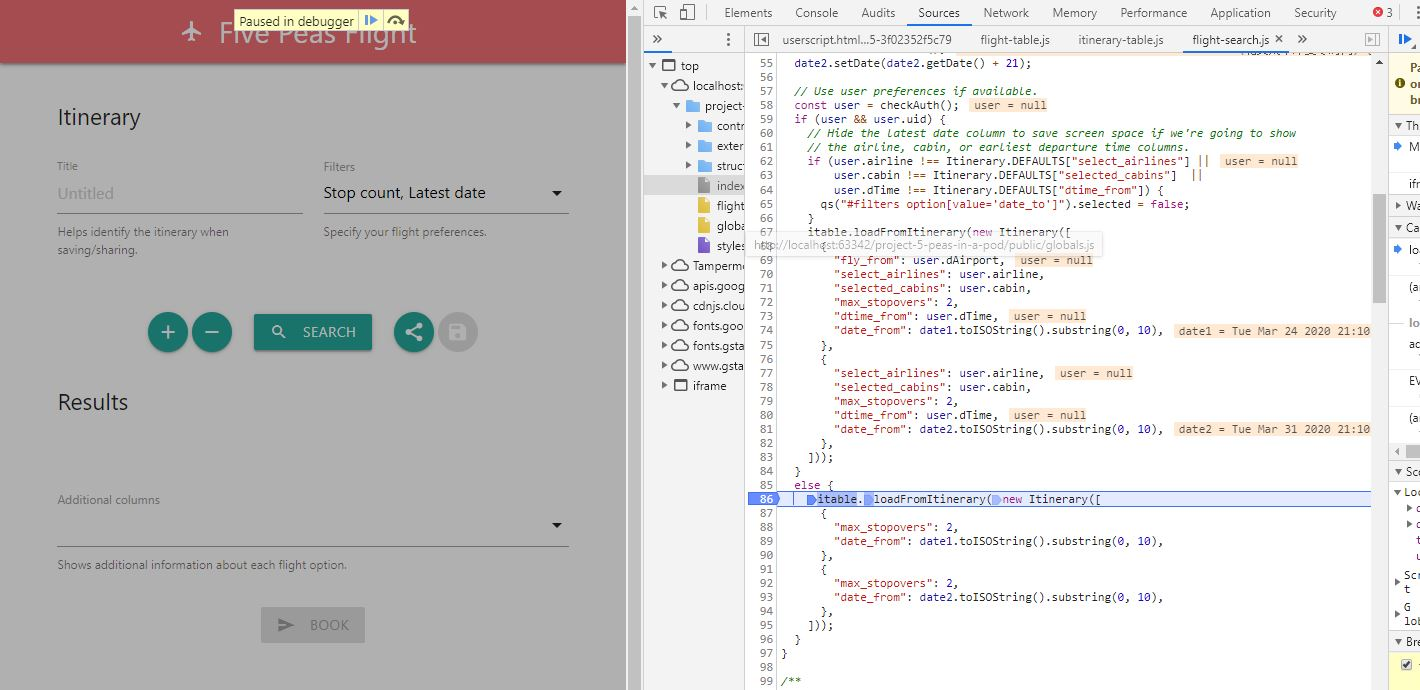
\includegraphics[width=\textwidth]{use-debugger.JPG}
% \caption{Before executing \code{itable.loadFromItinerary}, the search table is empty.}
% \label{fig:debugger}
% \end{figure}


% latex命令会忽略其后的空格,所以要加\ 或者{}。
\theproject\ loads a predefined list of airport names, and dash is used to separate airport name and airport code, for instance ``Los Angeles International Airport, Los Angeles, US - LAX''. In \path{public/control/itinerary-table.js}, 
\begin{lstlisting}
const trim = e => e.value = e.value.includes(" - ") ?
                  e.value.split(" - ")[1] : e.value;
\end{lstlisting}
is used to extract the airport code. However, itinerary-table.js has some airport names with multiple `` - '', as Figure \ref{fig:airport} shows. If a user searches these airports, the application cannot find any flights because of the wrong airport codes.

\begin{figure}[ht]
\centering
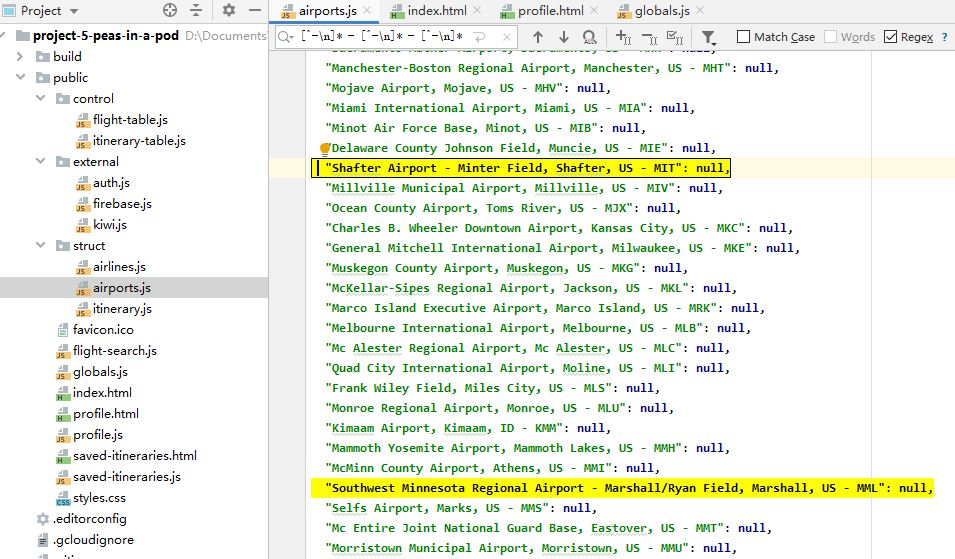
\includegraphics[width=\textwidth]{airport-names.JPG}
\caption{Airport names with multiple dashes break the search function.}
\label{fig:airport}
\end{figure}


\theproject\ stores partial authentication data, and user name and his preferences in browser local storage. Local storage does not expire and the user name may be leaked. It can be a privacy concern.



We then check the vulnerable candidate points founded in Section \ref{dependency-evaluation}.

\theproject\ uses the vulnerable components in Materialize, namely \code{autocomplete} and \code{tooltip}. Listing \ref{lst:autocomplete} and \ref{lst:tooltip} show two use sites. These contents are not user-generated. Therefore we think the risk is slow.

\begin{lstlisting}[frame=tb, caption=itinerary-table.js loads airlines to autocomplete, label=lst:autocomplete]
M.Autocomplete.init(autocomplete_select_airlines, {
  data: airlines,
  onAutocomplete: () => autocomplete_select_airlines.forEach(trim),
  limit: 5
});
\end{lstlisting}

\begin{lstlisting}[language=html, frame=tb, caption=itinerary-table.js loads airlines to tooltip, label=lst:tooltip]
<i class="material-icons tiny tooltipped" data-position="bottom"
    data-tooltip="${ItineraryTable.AIRPORT_TOOLTIP}<br><br>
    ${ItineraryTable.ORDER_FLEX_TOOLTIP}">info_outline</i>
\end{lstlisting}


\path{public/struct/itinerary.js} overwrites the native \code{escape} function, which was often used to escape HTML to plain text\textsuperscript{\cite{native-escape}}. The \code{escape} function implemented by the team does not cover all conditions required by ECMAScript 2020 Language Specification. Because of the discrepancies, external dependencies that use \code{escape} may become unstable, broken, or susceptible to arbitrary code execution vulnerability. Due to resource constraints, we didn't check the code of the dependencies. Nevertheless, we consider this as a high vulnerability.

\path{public/external/kiwi.js} has \code{itinerary.get(i, "fly\_from",\linebreak[4] false)}, which disables escaping of the value of field \code{fly\_from}. Although the current airport list doesn't have any HTML-like names, it would be good to run escaping, exercising defence in depth, and prevent future maintenance issues that a developer may accidentally put some HTML code into the list.

\subsubsection{Save Itinerary}
In this part, we focus on these 2 files - \code{public/saved-itineraries.html} and \code{public/saved-itineraries.js}. These 2 files are handling the saved itineraries webpage. \code{public/saved-itineraries.js} is responsible for supporting all user interactions with \code{saved-intineraries.html} page. If a user logged in his Google Account in the website, he could save his flight search results into history which was named by Saved Itineraries. The Saved Itineraries website is shown as figure \ref{fig:save_itineraries2}. 

\begin{figure}[ht]
\centering
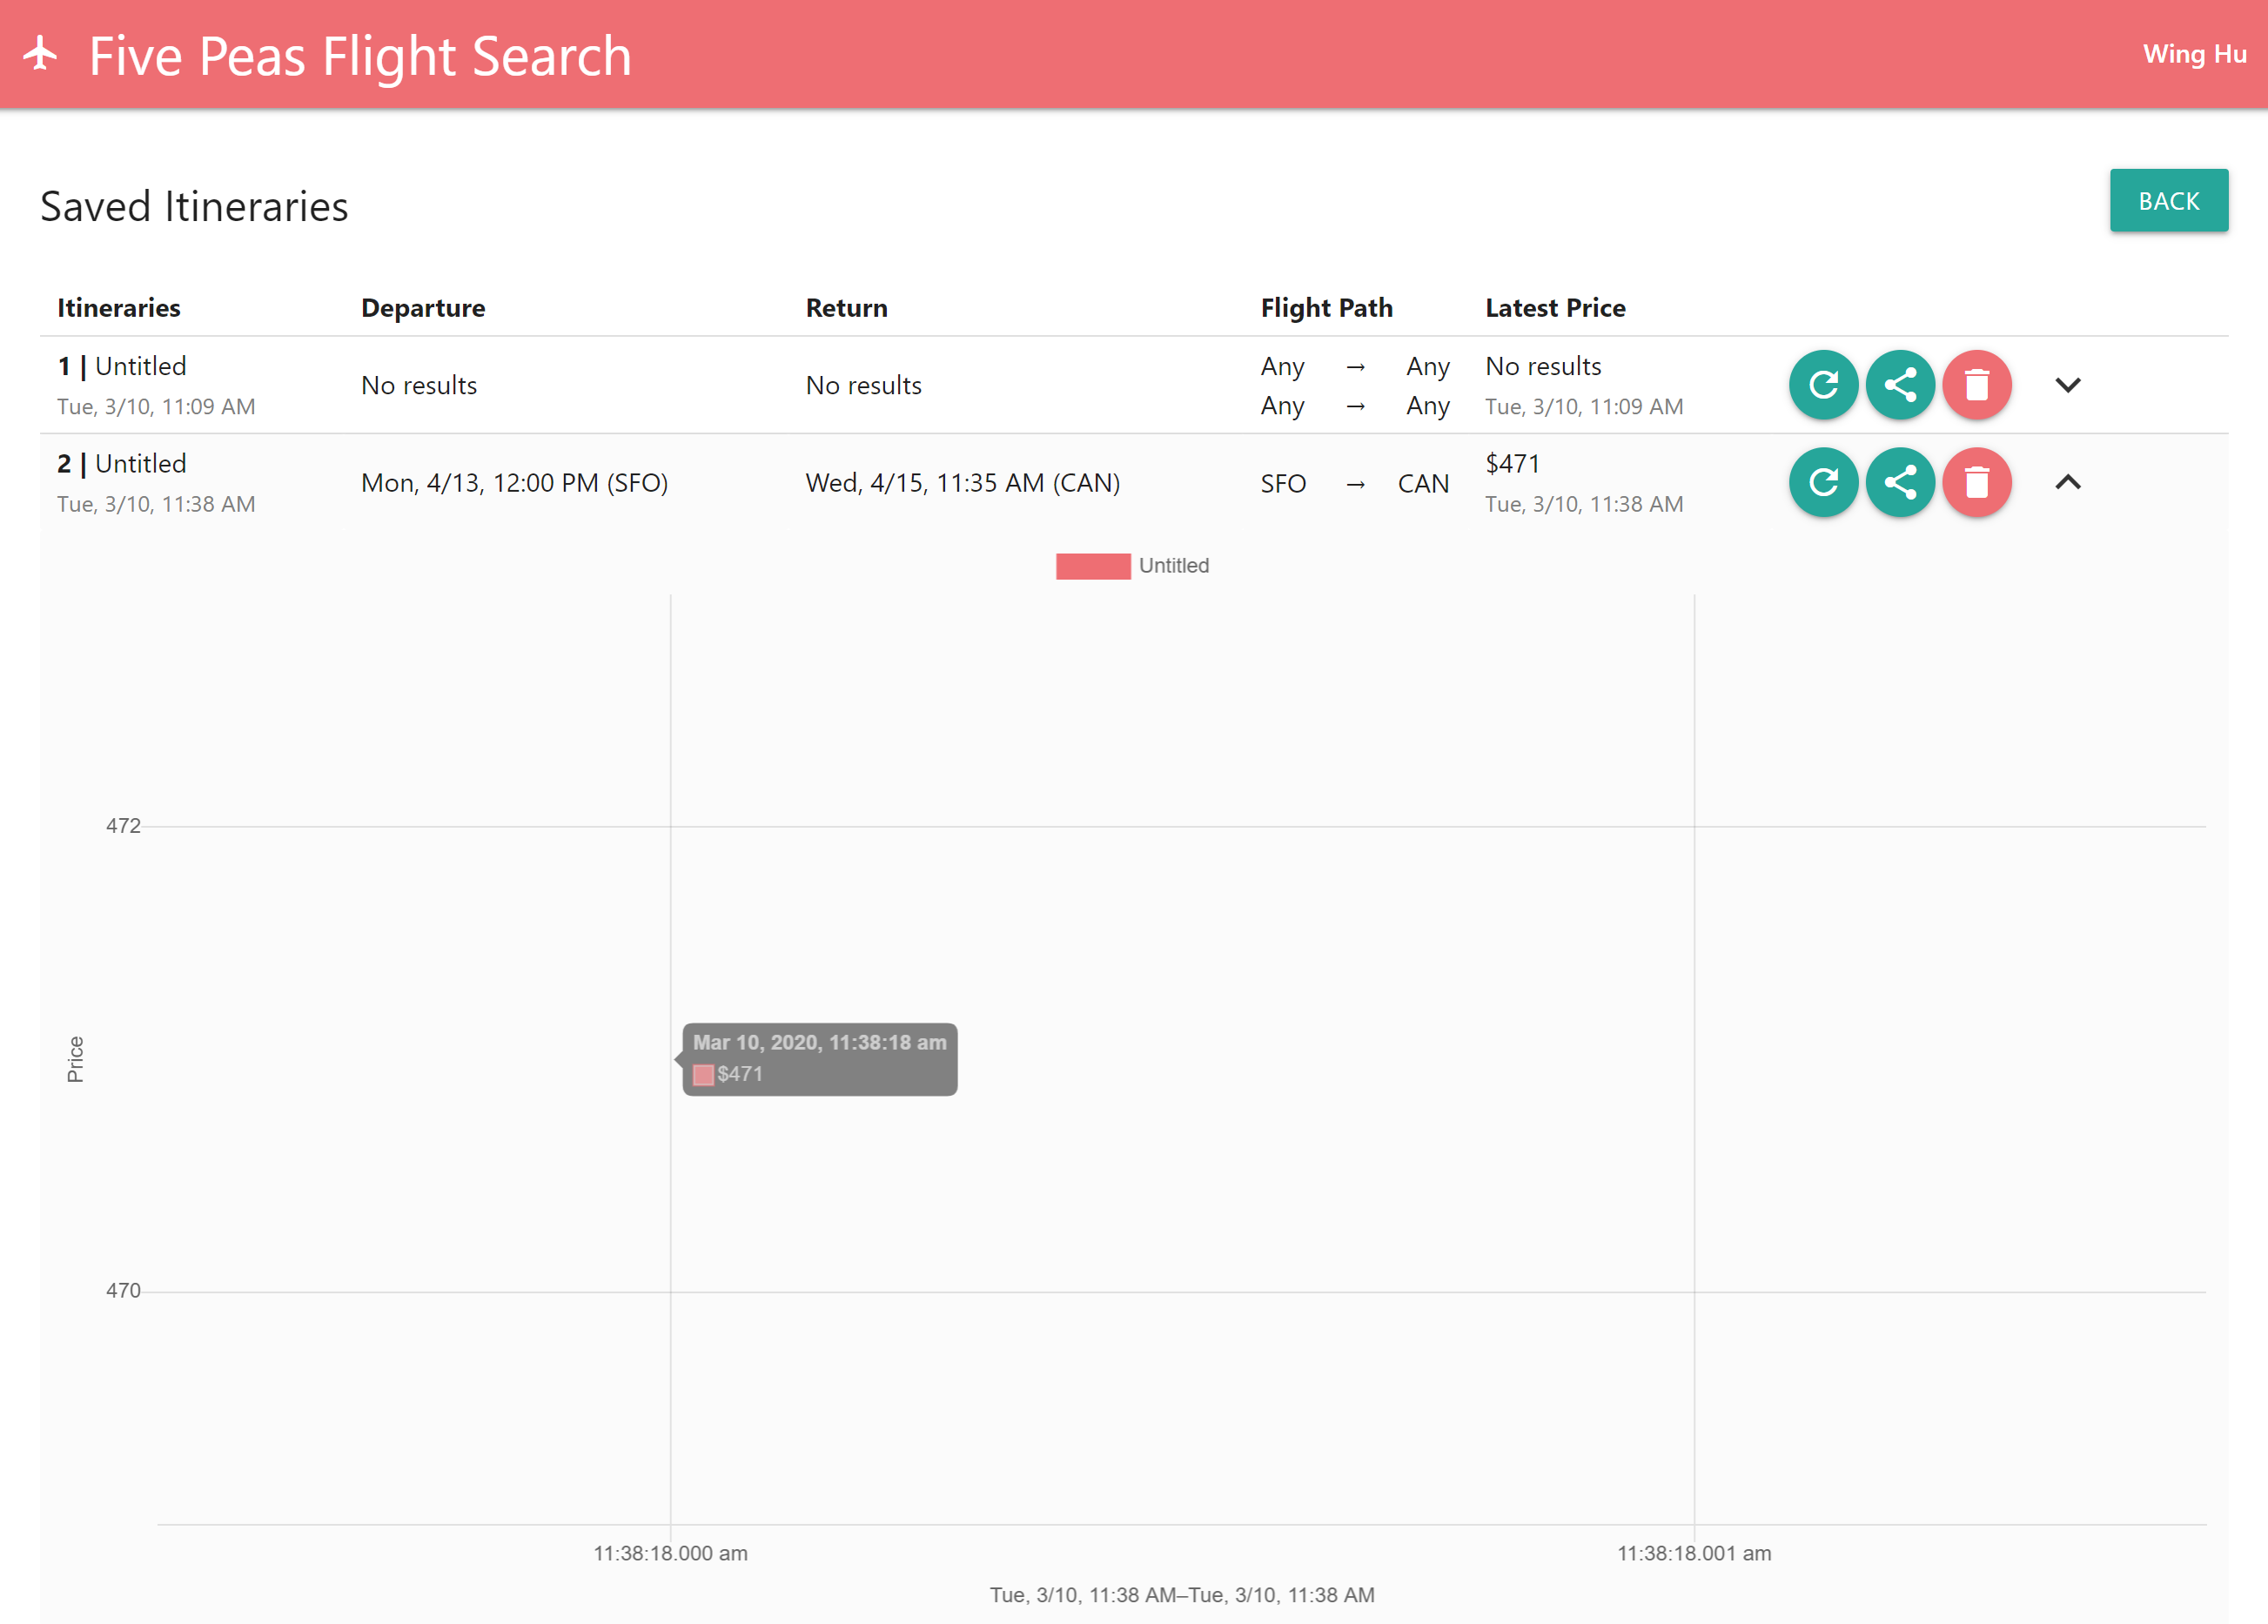
\includegraphics[width=\textwidth, frame]{save_itineraries2.png}
\caption{the UI of Save Itinerary}
\label{fig:save_itineraries2}
\end{figure}

\code{public/saved-itineraries.js} contains a lot of functions. For example, when a user is authorized, he can modify its data. On Listing \ref{lst:savedItineraries1} and \ref{lst:savedItineraries2}, it calls auth.js to check whether the user is authorized or not and calls firebase.js to handles the user's search history.

\begin{lstlisting}[frame=tb, caption=checks if user is authenticated with a call , label=lst:savedItineraries1]
addEventListener("load", () => {
  const user = checkAuth();
  if (!user || !user.uid) {
    qs("#itineraries-unauthenticated").classList.remove("hide");
    console.error("User is not authenticated.");
    return;
  }
\end{lstlisting}

\begin{lstlisting}[frame=tb, caption=Pulls user’s saved itineraries using call to firebase.js, label=lst:savedItineraries2]
getFirebaseItineraries(user.uid).then(data => {
    if (data.length === 0) {
      qs("#itineraries-authenticated").classList.add("hide");
      qs("#itineraries-none").classList.remove("hide");
    }
    else {
      sitable = new SavedItinerariesTable(data);
    }
  }).catch(error => {
    console.error(error);
    qs("#itineraries-authenticated").classList.add("hide");
    qs("#itineraries-none").classList.remove("hide");
  });
\end{lstlisting}

Furthermore, there are other functions in this file. Based on their project design(Figure \ref{}, I look through the module of each function, then make sure their description matches their function.

\begin{figure}[ht]
\centering
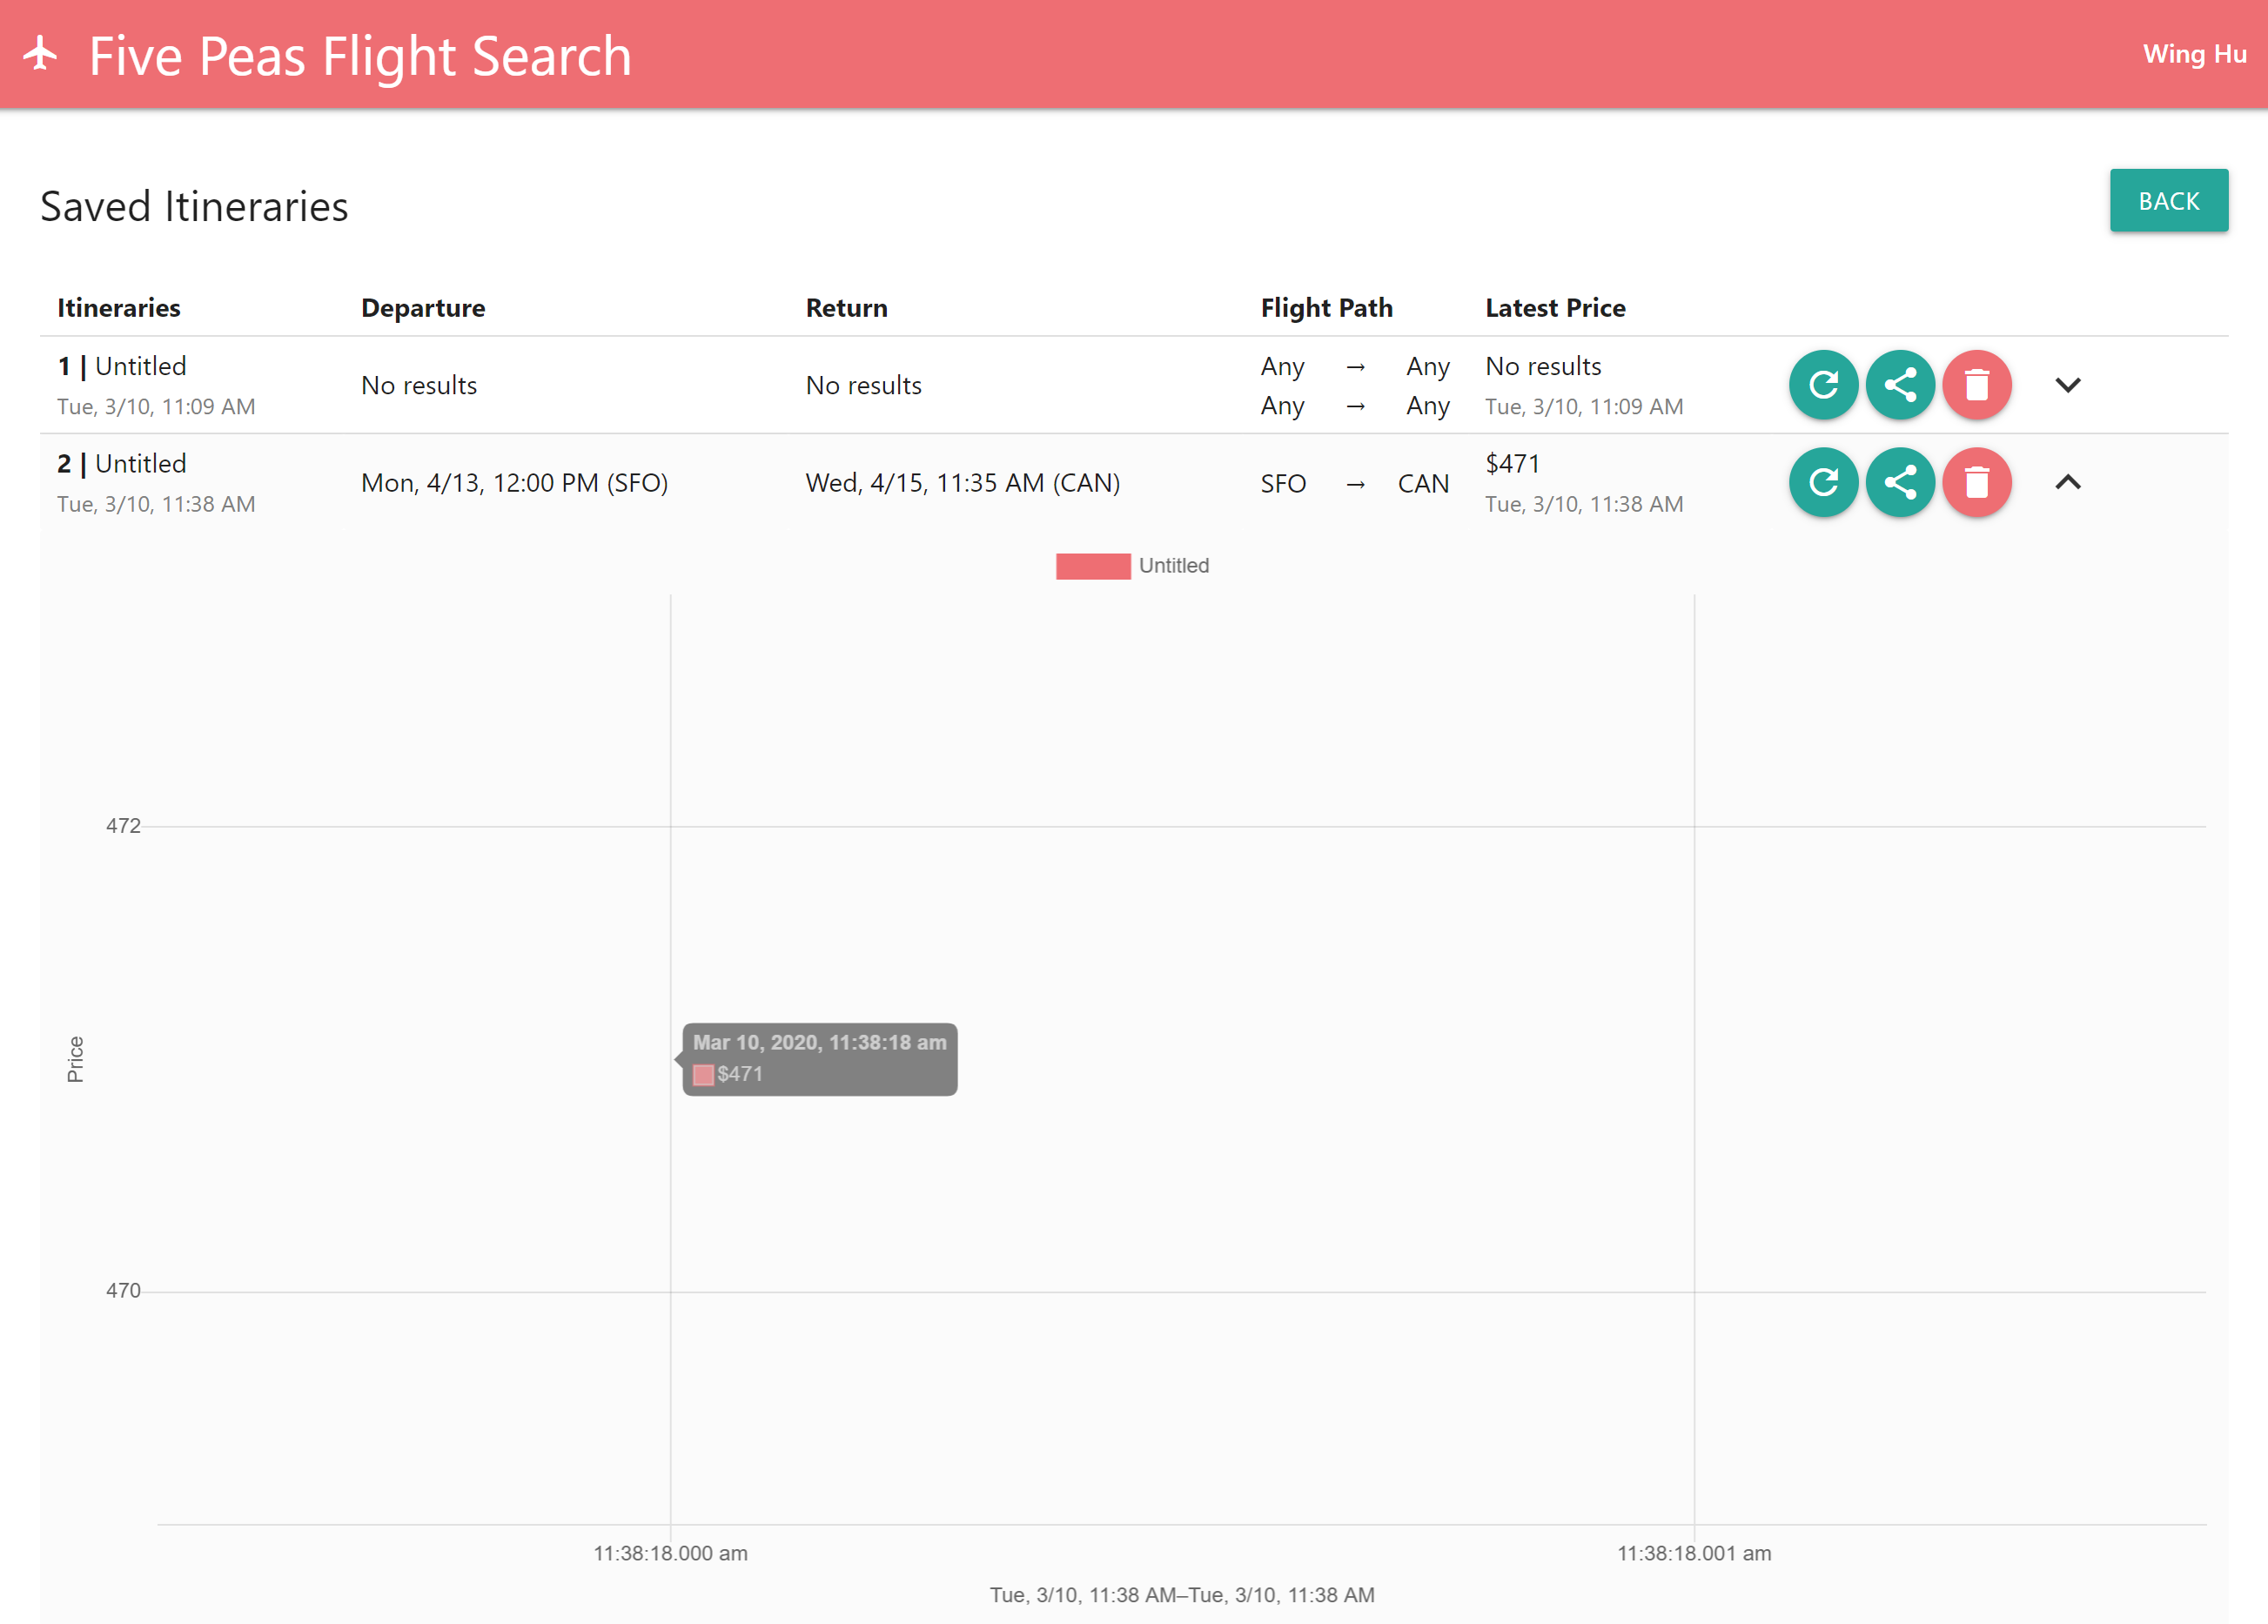
\includegraphics[width=\textwidth, frame]{save_itineraries2.png}
\caption{the UI of Save Itinerary}
\label{fig:save_itineraries2}
\end{figure}

We notice neither the input boxes on the home page have \code{maxlength}, nor does the JavaScript limit input length. When a user saves itinerary, the title can be super long. Five Peas in a Pod may set or Firebase has a default size limit on each itinerary, which is somewhere between 741 KB to 1 MB. This is too large in our opinion. 

\begin{figure}[ht]
\centering
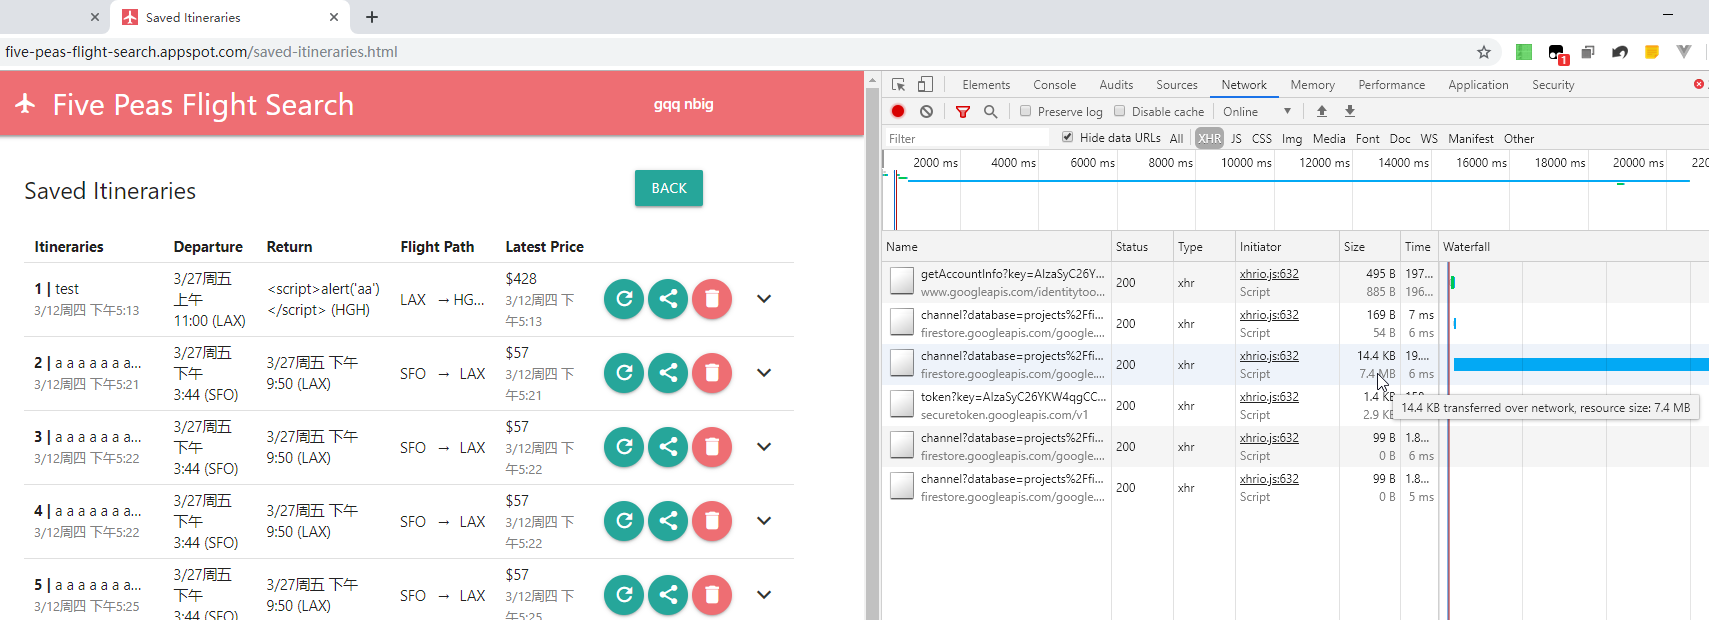
\includegraphics[width=\textwidth]{response-size.png}
\caption{Chrome developer tool verifies the server returns a page with 10 super long itineraries of total size 7.4 MB}
\label{fig:response-size}
\end{figure}

What's more, it's unclear how many itineraries one user can save. We saved more than 10 741KB-sized itineraries and did not reach a limit. When we visit the Saved Itineraries page, it pulled 7.4 MB from the server, as Figure \ref{fig:response-size} shows.

A malicious user can launch such attack with a large number of user accounts, eating up the storage space of \theproject\ or perform denial of service attack by slowing the server down.

Finally, loading a saved itinerary is by encoding the itinerary object as BASE64 and passing it through URL. Function \code{shareItinerary} in \path{public/globals.js} checks URL length with the code in Listing \ref{lst:url-length}, but the loading saved itinerary part doesn't. Hence, there is no way to load a large itinerary as Google App Engine server refuses such a long URL and resets the connection, even if saving large itinerary is allowed.

\begin{lstlisting}[frame=tb, caption=Sharing itinerary checks the length of URL, label=lst:url-length]
function shareItinerary(name, itinerary, button, hiddenInput) {
  button.classList.add("disabled");

  // Copy URL to clipboard if possible and set the message.
  let url = itinerary.link(name);
  let icon, message, color;
  if (url.length > 2048) {
    icon = "error";
    message = "Error: Itinerary is too long to share.";
    color = "red";
  }
  else {
    ...
\end{lstlisting}

\subsubsection{Log-in}
The log-in feature is supported by Google OAuth and mainly handled in \code{auth.js}, which deals with sign-in and sign-out logic. The users information is cached and stored in localStorage to update users' log-in status.
There are 7 interfaces: 
\code{gapiInit()} initializes Google sign-in and load Google OAuth Library. 
\code{auth()} check whether or not the Firebase auth status changes. If yes then remove the authentication state so that the user can no long have access to the stored data.
\code{checkAuth()} verifies the authentication status of a user.
\code{onLoadAuth()} handles the changes of the User Interface when the authentication status changes. It runs on DOMContentLoaded and sign in/sign out.
\code{isUserEqual()} would verify whether or not the Google account is the the same user of the Firebase account. If it's true, the users are able to access the stored information in Firebase.
\code{signup()} after a user logs in, this function creates a Firebase account for the specific user to store the information.
\code{signout()} execute when a user signs out.




%\subsection{Automated Tests}
%Project Google Play Advanced Search comes with a number of automated tests located in the tests module. These are all functional tests and the badge on the README file on the repository confirms the code passes all tests. However, there are no security tests there.


\subsection{Tool Testing Results}
\subsubsection{Nmap for Port Scanning}
We use Nmap to scan the open ports on the server. Currently the server has a public ip 172.217.5.212 and domain \code{five-peas-flight-search.\linebreak[1]appspot.com};

Running Nmap with \code{-T4 -A -v -p-} flag to scan 1000 most frequently used ports on the server.
We find ports 80, 443 are open. Port 80 (fig \ref{fig:nmap80}) is running http services and 
443 (fig \ref{fig:nmap443}) is running https services. No other open ports are found in these 1000 ports. Due to time limit, we didn't scan through all 66534 ports.

\begin{figure}[ht]
\centering
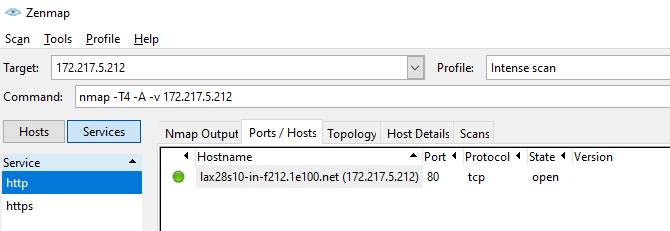
\includegraphics[width=0.8\textwidth, frame]{nmap80.png}
\caption{Port 80}
\label{fig:nmap80}
\end{figure}

\begin{figure}[ht]
\centering
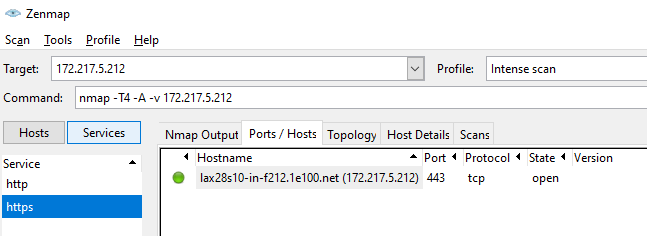
\includegraphics[width=0.8\textwidth, frame]{nmap443.png}
\caption{Port 443}
\label{fig:nmap443}
\end{figure}

\subsubsection{OWASP ZAP}
ZAP is a open source project developed by OWASP. It can help us to find the some potential security problems of our web server like SQL injection, XSS and many others.
We run zap to attack the website and found some Alerts:
\begin{itemize}
    \item Risk: \textcolor{orange}{medium}. CSP Scanner (fig \ref{fig:zap_csp}): Wildcard Directive under three urls below. It is usually caused by not defining default-src or frame-ancestor. We did a little research on Google App Engine and found that to avoid this vulnerability, default-src and frame-ancestor can be set in \code{app.yaml} which is currently not set.
    \begin{itemize}
        \item https://five-peas-flight-search.appspot.com/control
        \item https://five-peas-flight-search.appspot.com/external
        \item https://five-peas-flight-search.appspot.com/struct
    \end{itemize}
    
    \begin{figure}[ht]
    \centering
    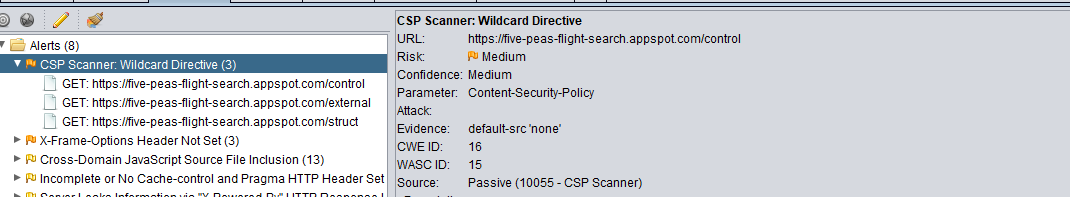
\includegraphics[width=\textwidth, frame]{zap_csp.png}
    \caption{Wildcard Directive}
    \label{fig:zap_csp}
    \end{figure}
    
    \item Risk: \textcolor{orange}{medium}. X-Frame-Options Header Not Set in three HTTP responses below (fig \ref{fig:zap_x}). Not including X-Frame-Optinons Header will cause less protection against ``ClickJacking'' attacks, also known as a “UI redress attack”, is when an attacker uses multiple transparent or opaque layers to trick a user into clicking on a button or link on another page when they were intending to click on the the top level page. Thus, the attacker is “hijacking” clicks meant for their page and routing them to another page, most likely owned by another application, domain, or both. Using a similar technique, keystrokes can also be hijacked. With a carefully crafted combination of stylesheets, iframes, and text boxes, a user can be led to believe they are typing in the password to their email or bank account, but are instead typing into an invisible frame controlled by the attacker.
    \begin{itemize}
        \item https://five-peas-flight-search.appspot.com/
        \item https://five-peas-flight-search.appspot.com/profile.html
        \item https://five-peas-flight-search.appspot.com/saved-itineraries.html
    \end{itemize}
    \begin{figure}[ht]
    \centering
    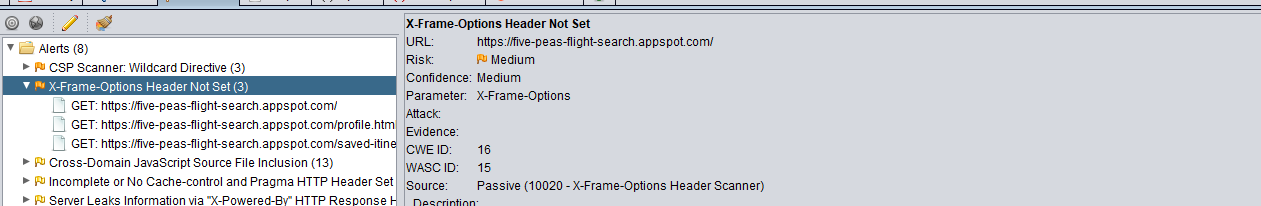
\includegraphics[width=\textwidth, frame]{zap_x.png}
    \caption{X-Frame-Options}
    \label{fig:zap_x}
    \end{figure}
    
    \item Risk: \textcolor{yellow}{low}. Cross-Domain JavaScript Source File Inclusion. Five-Peas-Flight-Search uses 13 scripts
    in total from third-party domain (fig \ref{fig:zap_cdjs}). There might be security issues when these third-party domain are attacked so the Five-Peas-Flight-Search are running some nasty codes. One could deploy the production mode of above third party JavaScript libraries to their own server to reduce the potential threat but it loses the benefits of content delivery network . 
    \begin{figure}[ht]
    \centering
    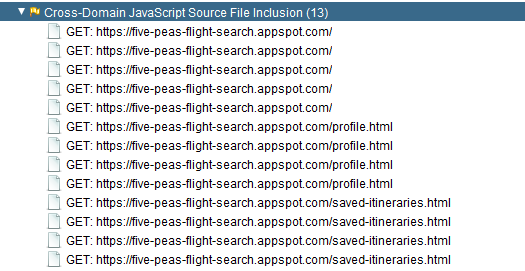
\includegraphics[width=\textwidth, frame]{zap_cdjs.png}
    \caption{Cross-Domain JavaScript Inclusion}
    \label{fig:zap_cdjs}
    \end{figure}
    
    \item Risk: \textcolor{yellow}{low}. Incomplete or No Cache-control and Pragma HTTP Header Set in four urls (fig \ref{fig:zap_cache_control}). The cache-control and pragma HTTP header have not been set properly or are missing allowing the browser and proxies to cache content.
    \begin{figure}[ht]
    \centering
    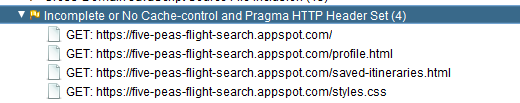
\includegraphics[width=\textwidth, frame]{zap_cache_control.png}
    \caption{Incomplete or No Cache-control and Pragma HTTP Header Set}
    \label{fig:zap_cache_control}
    \end{figure}

    \item Risk: \textcolor{yellow}{low}.  There are 25 Server Leaks Information via "X-Powered-By" HTTP Response Header Fields (fig: \ref{fig:zap_server_leak}). The web/application server is leaking information via one or more "X-Powered-By" HTTP response headers. Access to such information may facilitate attackers identifying other frameworks/components your web application is reliant upon and the vulnerabilities such components may be subject to.
    \begin{figure}[ht]
    \centering
    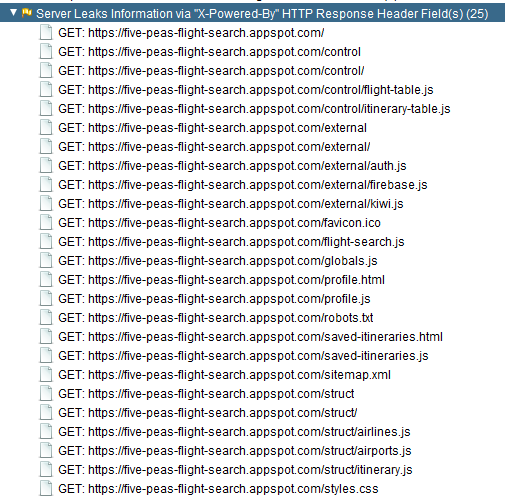
\includegraphics[width=\textwidth, frame]{zap_server_leak.png}
    \caption{Server Leaks Information}
    \label{fig:zap_server_leak}
    \end{figure}
    
    \item Risk: \textcolor{yellow}{low}. There 17 X-Content-Type-Options Header Missing (fig \ref{fig:zap_x_content}). 
    The Anti-MIME-Sniffing header X-Content-Type-Options was not set to 'nosniff'. This allows older versions of Internet Explorer and Chrome to perform MIME-sniffing on the response body, potentially causing the response body to be interpreted and displayed as a content type other than the declared content type. Version in early 2014 and legacy versions of Firefox will use the declared content type (if one is set), rather than performing MIME-sniffing.
    This issue still applies to error type pages (401, 403, 500, etc.) as those pages are often still affected by injection issues, in which case there is still concern for browsers sniffing pages away from their actual content type. At "High" threshold this scanner will not alert on client or server error responses.
    
    To avoid these vulnerabilities, one can ensure that the application/web server sets the Content-Type header appropriately, and that it sets the X-Content-Type-Options header to 'nosniff' for all web pages. If possible, ensure that the end user uses a standards-compliant and modern web browser that does not perform MIME-sniffing at all, or that can be directed by the web application/web server to not perform MIME-sniffing.

    \begin{figure}[ht]
    \centering
    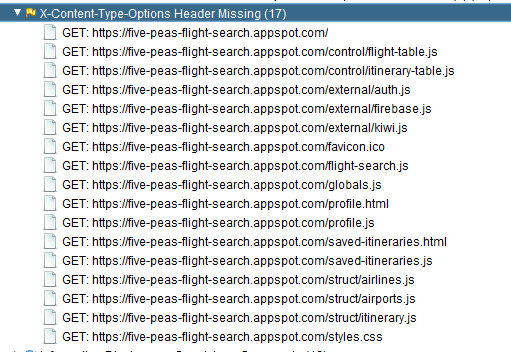
\includegraphics[width=\textwidth, frame]{zap_x_content.png}
    \caption{X-Content-Type-Options Header Missing}
    \label{fig:zap_x_content}
    \end{figure}
    
    \item Risk: \textcolor{blue}{Informational}. Information Disclosure - Suspicious Comments. The response appears to contain suspicious comments which may help an attacker. Note: Matches made within script blocks or files are against the entire content not only comments.
    \item Risk: \textcolor{blue}{Informational}. Timestamp Disclosure - Unix
\end{itemize}


\subsubsection{SSL Test}
We also use an online tool \code{immuniweb} to perform a ssl security check. See Figure \ref{fig:immuniweb}. The full result is available on \url{https://www.immuniweb.com/ssl/?id=teFxcVKZ} Although it has a good overall score, it still has some issues:

\begin{itemize}
    \item The server has TLS 1.0 enabled. Since the 30th of June 2018 it is non-compliant with PCI DSS
    \item Not providing OCSP Stapling.
    \item Some default ciphers from TSL 1.1 and 1.2 are non-compliant with HIPAA guidance or PCI DSS.
\end{itemize}

% For other two issues, we believe it's good to implement them on the server.


\begin{figure}[ht]
\centering
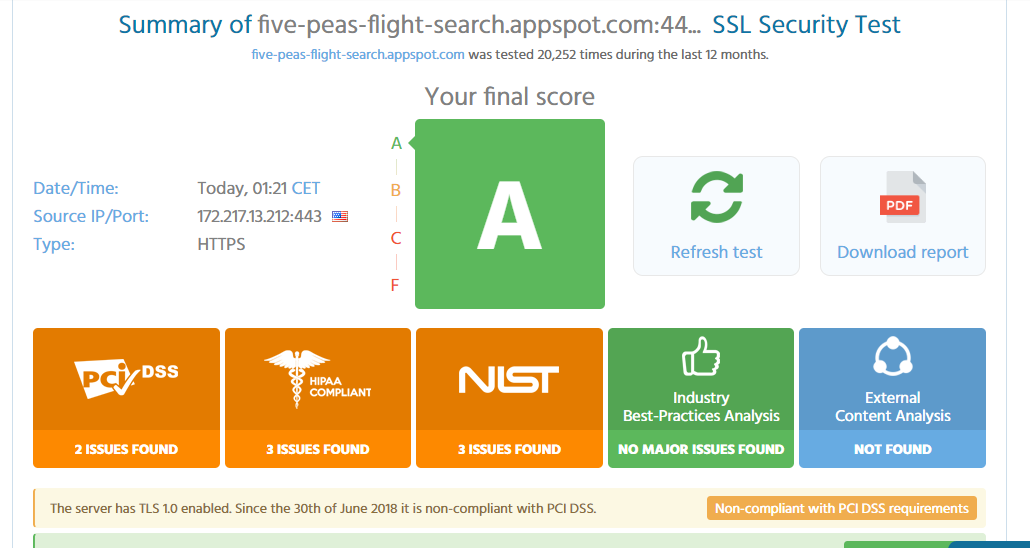
\includegraphics[width=0.7\textwidth]{immuniweb.png}
\caption{immuniweb.com gives A+ score on the server}
\label{fig:immuniweb}
\end{figure}

\section{Server Testing}
Five-Peas-Flight-Search is hosting on Google App Engine. To evaluate the server security we can pay attention to the configuration files that Five-Peas-Flight-Search provides to Google. Looking at the design document and code structure, we see that only these files are related to server configuration: \code{app.js} and \code{app.yaml}.

\subsection{Evaluating \code{app.js}}
The implementation uses \code{app.js} to recieve POST requests and response the desired context or status code if there is error. \code{app.js} verifies as well. The only data it can receive is the itineraries data and pass to firebase. It doesn't seem to have security issue on it. And it will be running on Google App Engine and we don't have connection access to the firebase, so we can not run some database security test tools like Scuba on it.

\subsection{Evaluating \code{app.yaml}}
See fig \ref{fig:app.yaml}. As stated above on the ZAP test analysis, \code{app.yaml} is not properly configured. In this configuration file, \code{default-src} and \code{frame-\linebreak[1] ancestor} are not set, but \code{secure} is set to \code{always}.
We did some research on it, and find out using \code{secure: always} redirects all HTTP traffic to an HTTPS URL with the same path. With \code{script: auto}, all traffic is served using the entrypoint command.


\begin{figure}[ht]
\centering
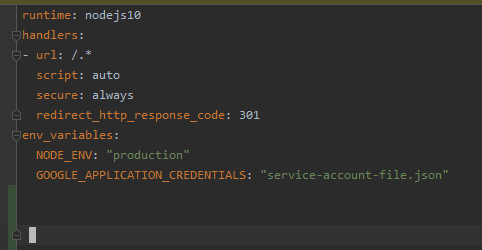
\includegraphics[width=\textwidth]{app_yaml.png}
\caption{app.yaml}
\label{fig:app.yaml}
\end{figure}

\subsection{Evaluating Google App Engine}
For internal access on server side, Google App Engine uses firewall to make internal network \code{Allow only traffic from within a specific network}, \code{Allow only traffic from a specific service
} and \code{Block abusive IP addresses}. As long as we trust 
the firewall, the vulnerabilities (like spoofing) on the server side is minimized if they don't change the firewall setting. In fact, we don't have the project ownership on Google Cloud and the configuration is not set by using configuration files. Performing a security test on firewall setting on server side is difficult. So we put it in future evaluation instead.



\section{Recommendations for future evaluations}

%Requirement: If time and resources did not permit you to study the system as fully as you feel was desirable, you should discuss how future efforts to better understand the security of the system should be directed. You should also discuss conditions under which a fresh review might be required, such as the addition of obvious major extensions to the prototype of the project. 

%Code review: Perform flow analysis carefully within functions you examine

We didn't look into JavaScript engine vulnerabilities this time. Future evaluation should look into that.

Future evaluation should check if external dependencies use the \code{escape} function because this native function is overwritten by the project.

\theproject\ uses Listing \ref{lst:parse-query-string} to parse query string parameters while the recommended and easier way is using the native \code{URLSearchParams} class\textsuperscript{\cite{URLSearchParams}}. Due to resource constraints, we didn't look into corner cases where the two algorithms produce different results.

\begin{lstlisting}[frame=tb, caption=parse query string parameters by regular expression, label=lst:parse-query-string]
let urlParams = {};
window.location.search.replace(/[?&]+([^=&]+)=([^&]*)/gi, (_, k, v) =>
            urlParams[k] = decodeURIComponent(v));
\end{lstlisting}

If we have the ownership of the project, We can also perform a Security scanner provided by Google. The Google Cloud Security Scanner discovers vulnerabilities by crawling App Engine app, following all that links within the scope of the starting URLs, and attempting to exercise as many user inputs and event handlers as possible.  Since we didn't know about this tool, so we didn't ask for the ownership of the project on Google Cloud. And it can find out if the firewall has safe setting.


\section{Lessons learned by performing the security evaluation}

When we found the maxlength issue in \theproject, we realize we didn't add the maxlength attribute to our own project either. However, our project doesn't store direct user input, so the impact is smaller.

We learned comments are very important. \theproject\ has plenty of comments, which helped us understand the system better and easier. 

We learned using \code{const} to declare variables can make the system more secure. \theproject\ uses it in some critical places, so we are unable to manipulate the variable value to bypass security checks.

We learned that the way they used Google Cloud to server content to the clients is a great way to ensure the security of user's information. Since in this way, Google has provided the guaranteed security in DDos protection and secure token generation, it is much easier and safer than creating a new database to store user privacy information. 

\section{Work breakdown}
Qiqi Gu - responsible for External Components Evaluation, part of Code Review, and proofreading. He found the overwritten escape vulnerability, maxlength and storage vulnerability, and some glitches.

Dongyao Liang - responsible to use tools to test our security and evaluate our server.

Shuhua Zhan - responsible for lessons learned section of the report and participated in code review. 

Yingze Hu - responsible for security design review.

Weikeng Yang - responsible for using tool to test the security and lessons learned section. 




\pgfkeys{
 /citeWeb/.is family, /citeWeb,
 date/.estore in = \citeWebdate,
}

\newcommand{\citeWeb}[4][date=]{\pgfkeys{/citeWeb, #1}%
#2, \url{#3}, %
\ifx\citeWebdate\empty\else\citeWebdate, \fi%
Retrieved #4.}

\begin{thebibliography}{99}
    \bibitem{chrome-update} \citeWeb{Stable Channel Update for Desktop}{https://chromereleases.googleblog.com/2020/02/stable-channel-update-for-desktop_24.html}{2020-03-10}
    \bibitem{secure-javascript} \citeWeb[date=2018-01-18]{Building Secure JavaScript Applications}{https://nemethgergely.com/building-secure-javascript-applications/}{2020-03-10}
    \bibitem{materialize-vulnerabilities} \citeWeb{Vulnerability report for materialize-css@1.0.0}{https://snyk.io/test/npm/materialize-css/1.0.0}{2020-03-10}
    \bibitem{google-fonts-privacy} \citeWeb[date=2019-11-28]{A privacy concern about Google Fonts
}{https://uxdesign.cc/a-privacy-concern-about-google-fonts-5aa4418bf87e}{2020-03-10}
    \bibitem{native-escape} \citeWeb{ECMAScript® 2020 Language Specification}{https://tc39.es/ecma262/\#sec-escape-string}{2020-03-10}
    \bibitem{URLSearchParams} \citeWeb{URL
Living Standard}{https://url.spec.whatwg.org/\#urlsearchparams}{2020-03-12}
    \bibitem{Google-DDoS}\citeWeb{Google Cloud Platform}{https://cloud.google.com/files/GCPDDoSprotection-04122016.pdf}{2020-03-09}
    \bibitem{firebase} \citeWeb{Full-Stack Firebase}{https://www.fullstackfirebase.com/cloud-firestore/security-rules}{2020-03-09}
    \bibitem{Google-Firebase-security} \citeWeb{Google Firebase security Bypassed}{https://searchsecurity.techtarget.com/answer/How-was-Google-Firebase-security-bypassed}{2020-03-13}    
\end{thebibliography}


%\section{Supplementary materials}
%Requirement: If your analysis produced useful artifacts (such as automated reports, screen shots demonstrating problems, scripts used to test functionality, etc.), include these in appendices, where possible. For things that are not easily embedded in a 
%report (such as a video demonstrating how to exploit a security flaw), upload them as separate files when you submit the report. You can also provide links to supplementary materials, but if you do, make sure that the materials are in a location that can be accessed by others, not in a private area. Make sure that your supplementary material section indicates which files are uploaded as part of your report, which links are associated with your report, and what each file or link represents.  
% 

\end{document}